\chapter{Lösung der Praktikumsaufgabe}
\section{Verwendung der REST-API mithilfe des Tools cURL}
\begin{enumerate}
	\item Lernen Sie das Tool cURL kennen
		\begin{description}
			\item[-v, --verbose] Stellt weitere Informationen zum abgesendeten Request, unter anderem gesendete bzw. empfangene \gls{HTTP}-Header, bereit. Mit \enquote{>} beginnende Zeilen stellen gesendete und mit einem \enquote{<} beginnende Zeilen stellen empfangene Header dar.
			\item[-H, --header] Mithilfe dieses Parameters lassen sich weitere \gls{HTTP}-Header definieren, welche dem Request hinzugefügt werden sollen.
			\item[-X, --request] Definiert den zu verwendenden Request-Typ, welcher für die Kommunikation mit dem Server verwendet werden soll.  
			\item[-d, --data] Spezifiziert die Daten, welche mittels POST-Request gesendet werden sollen. Ist dieser Parameter gesetzt wird der Request-Typ POST automatisch gewählt.
		\end{description}
	\item Bedeutung der HTTP-Methoden
		\begin{description}
			\item[OPTIONS] Die Methode OPTIONS wird dazu verwendet, um die Optionen der Kommunikation für die Zielressource zu beschreiben.
			\item[GET] Mithilfe dieser Methode wird eine Präsentation einer Ressource angefordert. Dabei sollte sie nur dazu genutzt werden, um Daten abzufragen.
			\item[HEAD] Mit dieser Methode wird dieselbe Anfrage wie mit einem GET-Request gestellt, jedoch wird der Antworttext nicht mitgesendet.
			\item[POST] Diese Methode dient zur Übermittlung von Daten an die angegebene Ressource, was häufig Statusänderungen oder anderweitige Nebenwirkungen nach sich zieht. 
			\item[PUT] Mithilfe dieser Methode werden alle Daten einer Ressource, durch die übermittelten Daten ersetzt.
			\item[PATCH] Mit dieser Methode lassen sich partielle Änderungen an einer Ressource vornehmen.
			\item[DELETE] Ein Aufruf dieser Methode führt zur Löschung der angegebenen Ressource.
		\end{description}
	\newpage
	\item Navigation durch die \gls{REST}-\gls{API}
		\begin{itemize}
			\item curl -sSL -D - localhost:8080/api -o /dev/null\\
				\\
				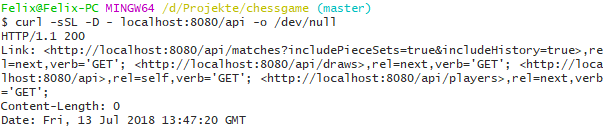
\includegraphics[width=0.8\textwidth]{images/question3.1.png}
			\item curl -sSL -D - localhost:8080/api/players -o /dev/null\\
				\\
				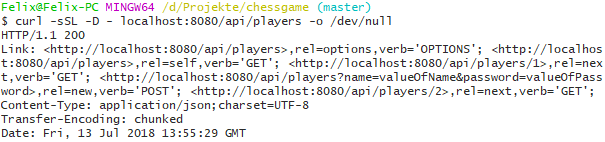
\includegraphics[width=0.8\textwidth]{images/question3.2.png}
			\item curl -sSL -D - localhost:8080/api/players/2 -o /dev/null\\
				\\
				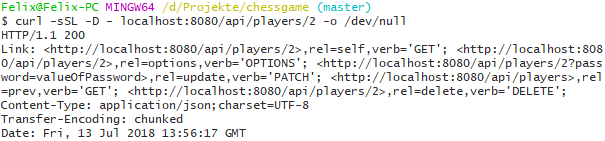
\includegraphics[width=0.8\textwidth]{images/question3.3.png}
			\item curl -sSL -D - localhost:8080/api/players -o/dev/null
			\item curl -sSL -D - localhost:8080/api -o /dev/null
			\item curl -sSL -D - localhost:8080/api/matches -o /dev/null\\
				\\
				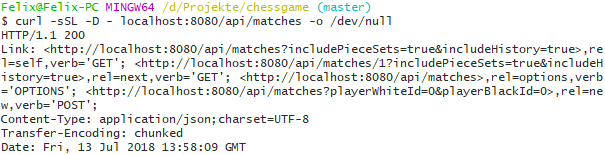
\includegraphics[width=0.8\textwidth]{images/question3.6.png}
			\newpage
			\item curl -sSL -D - localhost:8080/api/matches/1 -o /dev/null\\
				\\
				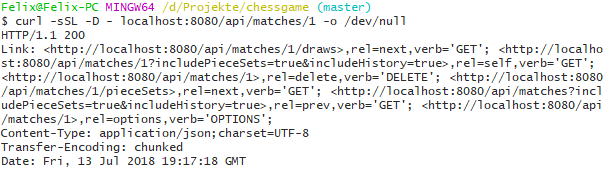
\includegraphics[width=0.8\textwidth]{images/question3.7.png}
			\item curl -sSL -D - localhost:8080/api/matches/1/draws -o /dev/null\\
				\\
				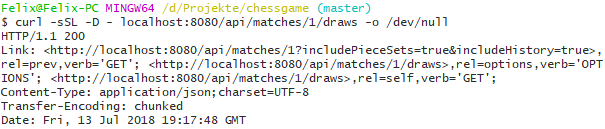
\includegraphics[width=0.8\textwidth]{images/question3.8.png}
			\item curl -sSL -D - localhost:8080/api/matches/1 -o /dev/null
			\item curl -sSL -D - localhost:8080/api/matches/1/pieceSets -o /dev/null\\
				\\
				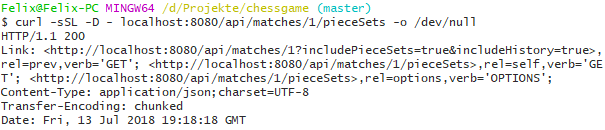
\includegraphics[width=0.8\textwidth]{images/question3.10.png}
			\item curl -sSL -D - localhost:8080/api/matches/1 -o /dev/null
			\item curl -sSL -D - localhost:8080/api/matches -o /dev/null
			\item curl -sSL -D - localhost:8080/api -o /dev/null
			\item curl -sSL -D - localhost:8080/api/draws -o /dev/null\\
				\\
				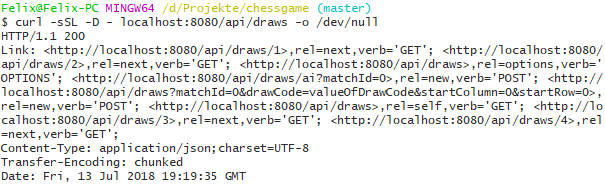
\includegraphics[width=0.8\textwidth]{images/question3.14.png}
			\newpage
			\item curl -sSL -D - localhost:8080/api/draws/1 -o /dev/null\\
				\\
				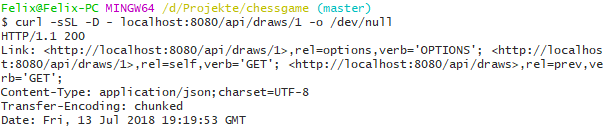
\includegraphics[width=0.8\textwidth]{images/question3.15.png}
			\item curl -sSL -D - localhost:8080/api/draws -o /dev/null
			\item curl -sSL -D - localhost:8080/api -o /dev/null
		\end{itemize}
	\item Anlegen neuer Player
		\begin{itemize}
			\item curl -v -H \textquotesingle Content-Type: application/x-www-form-urlencoded\textquotesingle\\-d \textquotesingle name=Test\&password=123456\textquotesingle\ localhost:8080/api/players\\
				\\
				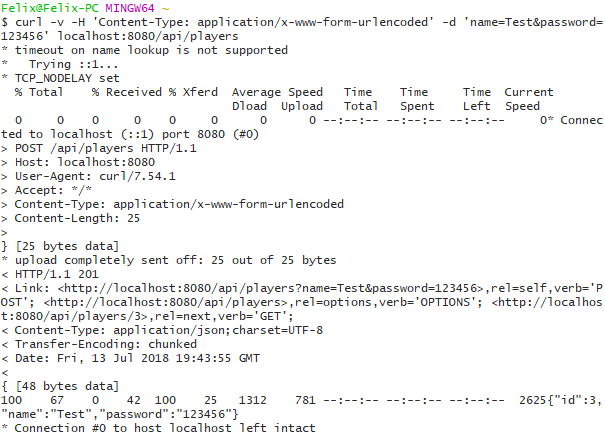
\includegraphics[width=0.8\textwidth]{images/question4.1.png}
			\newpage
			\item curl -v -H \textquotesingle Content-Type: application/json\textquotesingle\\-d \textquotesingle\{ "name": "Test", "password": "123456"\ \}\textquotesingle\ localhost:8080/api/players\\
				\\
				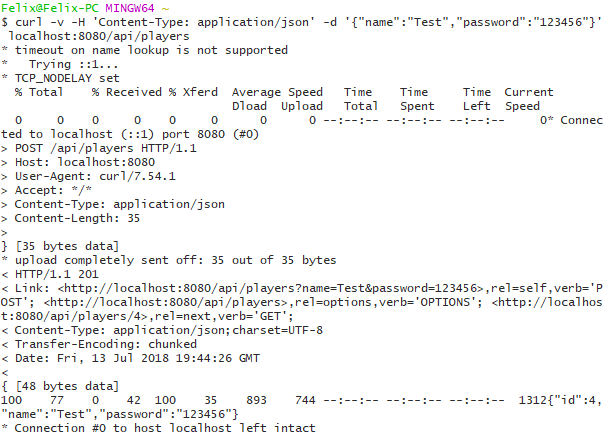
\includegraphics[width=0.8\textwidth]{images/question4.2.png}
		\end{itemize}
	\item Aktualisierung eines Players
		\begin{itemize}
			\item curl -v -X PATCH -H \textquotesingle Content-Type: application/json\textquotesingle\\-d \textquotesingle\{ "password": "987654"\ \}\textquotesingle\ localhost:8080/api/players/3\\
				\\
				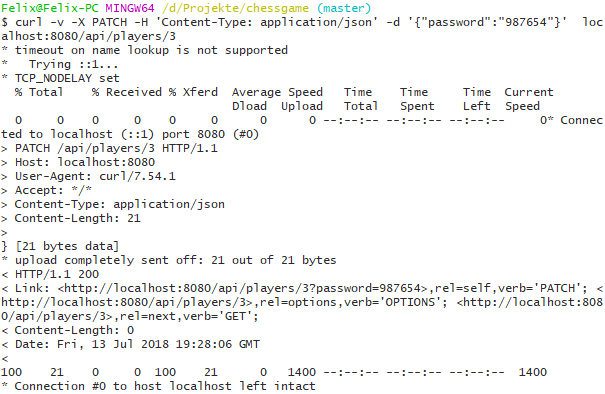
\includegraphics[width=0.8\textwidth]{images/question5.png}
		\end{itemize}
	\newpage
	\item Löschen eines Players
		\begin{itemize}
			\item curl -v -X DELETE localhost:8080/api/players/3\\
				\\
				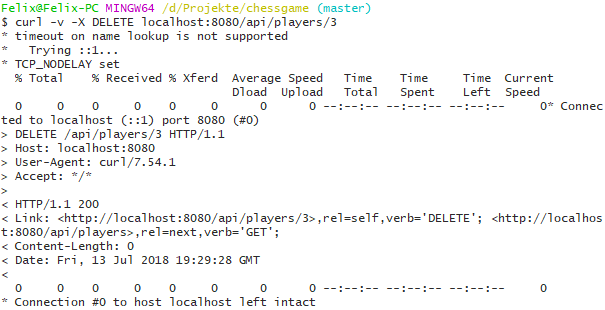
\includegraphics[width=0.8\textwidth]{images/question6.png}
		\end{itemize}
	\newpage
	\item Anlegen eines neuen Matches
		\begin{itemize}
			\item curl -v -H \textquotesingle Content-Type: application/json\textquotesingle\\-d \textquotesingle\{ "playerWhiteId": 1, "playerBlackId": 2\ \}\textquotesingle\ localhost:8080/api/matches\\
				\\
				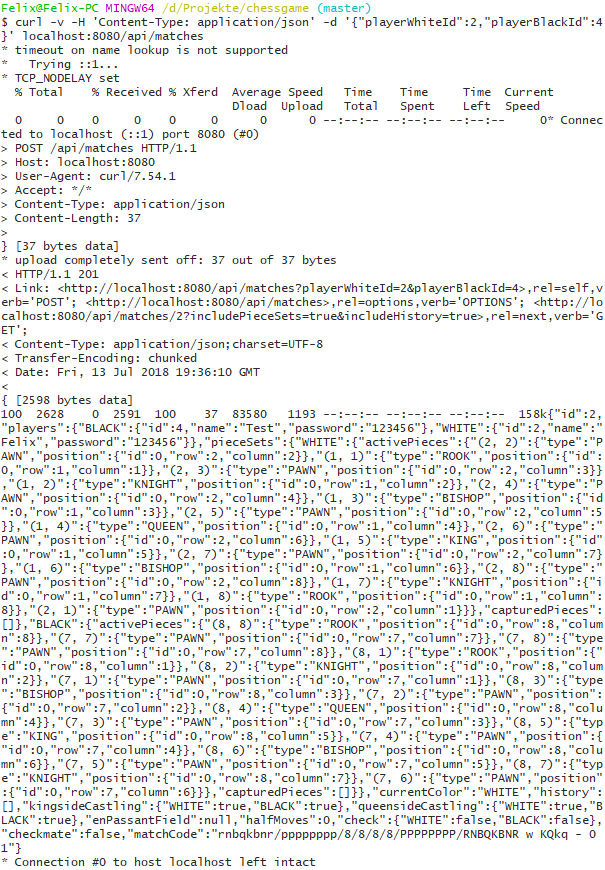
\includegraphics[width=0.8\textwidth]{images/question7.png}
		\end{itemize}
	\newpage
	\item Anlegen neuer Draws
		\begin{itemize}
			\item curl -v -H \textquotesingle Content-Type: application/json\textquotesingle\\-d \textquotesingle\{ "matchId": 2, "drawCode": \textquotesingle\textquotesingle e4", \textquotesingle\textquotesingle startColumn": 5, \textquotesingle\textquotesingle startRow": 2\ \}\textquotesingle\\localhost:8080/api/draws\\
				\\
				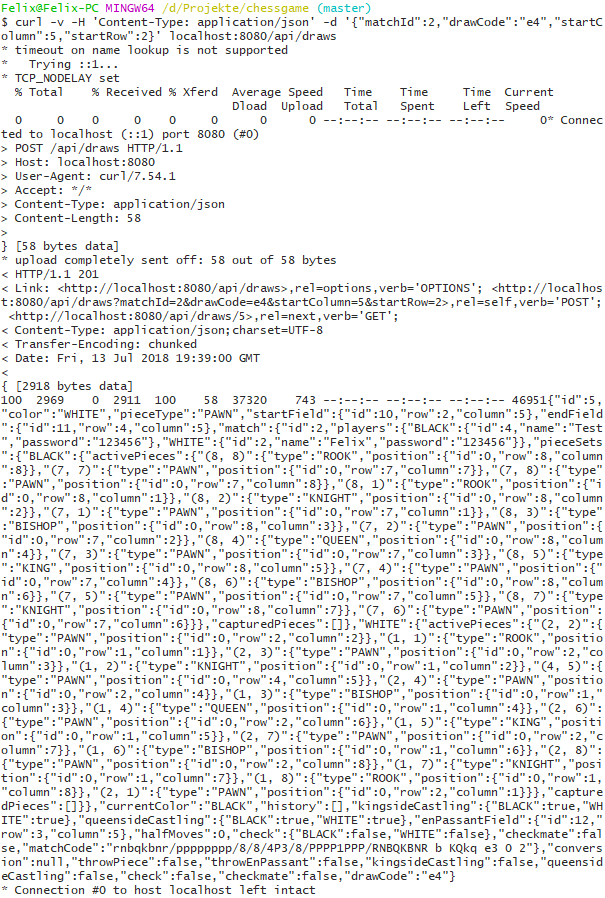
\includegraphics[width=0.8\textwidth]{images/question8.1.png}
			\newpage
			\item curl -v -H \textquotesingle Content-Type: application/json\textquotesingle\\-d \textquotesingle \{ "matchId": 2, "drawCode": "d5", \textquotesingle\textquotesingle startColumn": 4, \textquotesingle\textquotesingle startRow": 7\ \}\textquotesingle\\localhost:8080/api/draws\\
				\\
				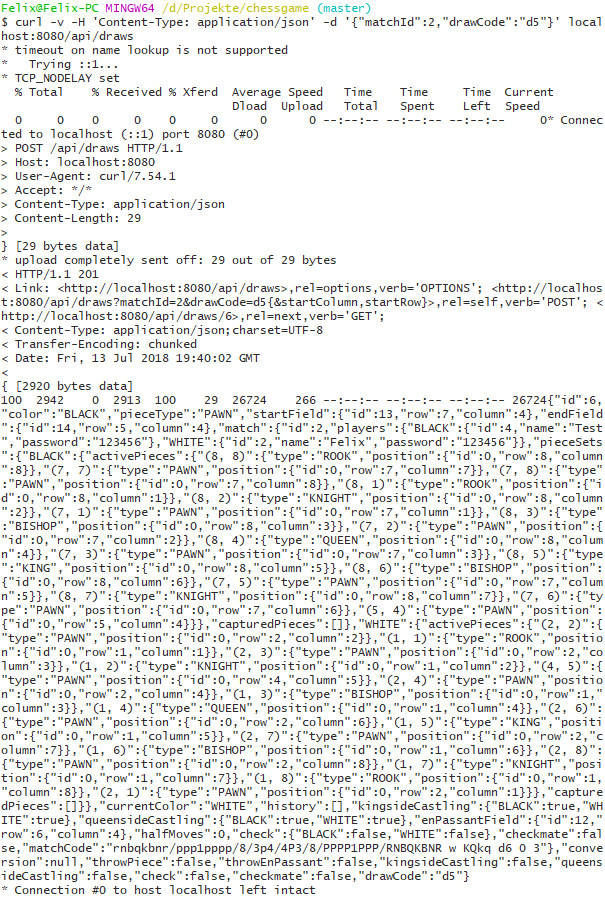
\includegraphics[width=0.8\textwidth]{images/question8.2.png}
			\newpage
			\item curl -v -H \textquotesingle Content-Type: application/json\textquotesingle\\-d \textquotesingle \{ "matchId": 2, "drawCode": \textquotesingle\textquotesingle exd5", \textquotesingle\textquotesingle startColumn": 5, \textquotesingle\textquotesingle startRow": 4\ \}\textquotesingle\\localhost:8080/api/draws\\
				\\
				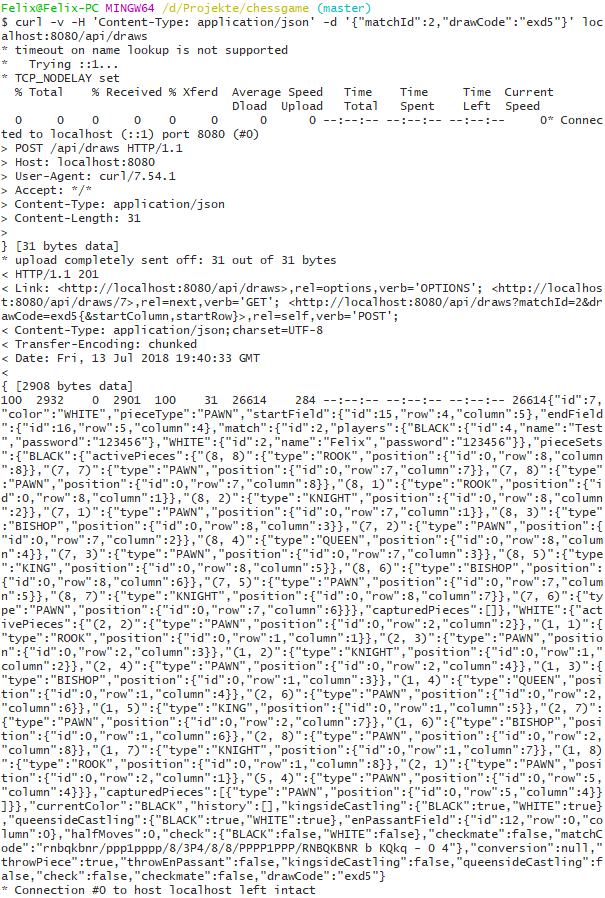
\includegraphics[width=0.8\textwidth]{images/question8.3.png}
		\end{itemize}
\end{enumerate}